\documentclass[a4paper,twoside]{article}
\usepackage{blindtext}  
\usepackage{geometry}

% Chinese support
\usepackage[UTF8, scheme = plain]{ctex}

% Page margin layout
\geometry{left=2.3cm,right=2cm,top=2.5cm,bottom=2.0cm}


\usepackage{listings}
\usepackage{xcolor}
\usepackage{geometry}
\usepackage{amsmath}
\usepackage{float}
\usepackage{hyperref}

\usepackage{graphics}
\usepackage{graphicx}
\usepackage{epsfig}
\usepackage{float}

\usepackage{algorithm}
\usepackage[noend]{algpseudocode}

\usepackage{booktabs}
\usepackage{threeparttable}
\usepackage{longtable}
\usepackage{listings}
\usepackage{tikz}
\usepackage{multicol}

\usepackage{caption}
\usepackage{subcaption}

% cite package, to clean up citations in the main text. Do not remove.
\usepackage{cite}

\usepackage{color,xcolor}

%% The amssymb package provides various useful mathematical symbols
\usepackage{amssymb}
%% The amsthm package provides extended theorem environments
\usepackage{amsthm}
\usepackage{amsfonts}
\usepackage{enumerate}
\usepackage{enumitem}
\usepackage{listings}

\usepackage{indentfirst}
\setlength{\parindent}{2em} % Make two letter space in the first paragraph
\usepackage{setspace}
\linespread{1.5} % Line spacing setting
\usepackage{siunitx}
\setlength{\parskip}{0.5em} % Paragraph spacing setting

% \usepackage[contents =22920202204622, scale = 10, color = black, angle = 50, opacity = .10]{background}

\renewcommand{\figurename}{图}
\renewcommand{\lstlistingname}{代码} 
\renewcommand{\tablename}{表格}
\renewcommand{\contentsname}{目录}
\floatname{algorithm}{算法}

\graphicspath{ {images/} }

%%%%%%%%%%%%%
\newcommand{\StudentNumber}{22920202204622}  % Fill your student number here
\newcommand{\StudentName}{熊恪峥}  % Replace your name here
\newcommand{\PaperTitle}{实验(二) timewrite:同步写与异步写}  % Change your paper title here
\newcommand{\PaperType}{Unix程序设计} % Replace the type of your report here
\newcommand{\Date}{2022年10月7日}
\newcommand{\College}{信息学院}
\newcommand{\CourseName}{Unix程序设计}
%%%%%%%%%%%%%

%% Page header and footer setting
\usepackage{fancyhdr}
\usepackage{lastpage}
\pagestyle{fancy}
\fancyhf{}
% This requires the document to be twoside
\fancyhead[LO]{\texttt{\StudentName }}
\fancyhead[LE]{\texttt{\StudentNumber}}
\fancyhead[C]{\texttt{\PaperTitle }}
\fancyhead[R]{\texttt{第{\thepage}页,共\pageref*{LastPage}页}}


\title{\PaperTitle}
\author{\StudentName}
\date{\Date}

\lstset{
	basicstyle          =   \sffamily,          % 基本代码风格
	keywordstyle        =   \bfseries,          % 关键字风格
	commentstyle        =   \rmfamily\itshape,  % 注释的风格,斜体
	stringstyle         =   \ttfamily,  % 字符串风格
	flexiblecolumns,                % 别问为什么,加上这个
	numbers             =   left,   % 行号的位置在左边
	showspaces          =   false,  % 是否显示空格,显示了有点乱,所以不现实了
	numberstyle         =   \zihao{-5}\ttfamily,    % 行号的样式,小五号,tt等宽字体
	showstringspaces    =   false,
	captionpos          =   t,      % 这段代码的名字所呈现的位置,t指的是top上面
	frame               =   lrtb,   % 显示边框
}

\lstdefinestyle{PythonStyle}{
	language        =   Python, % 语言选Python
	basicstyle      =   \zihao{-5}\ttfamily,
	numberstyle     =   \zihao{-5}\ttfamily,
	keywordstyle    =   \color{blue},
	keywordstyle    =   [2] \color{teal},
	stringstyle     =   \color{magenta},
	commentstyle    =   \color{red}\ttfamily,
	breaklines      =   true,   % 自动换行,建议不要写太长的行
	columns         =   fixed,  % 如果不加这一句,字间距就不固定,很丑,必须加
	basewidth       =   0.5em,
}

\lstdefinestyle{MakefileStyle}{
	otherkeywords={.SUFFIXES},
	morekeywords={SUFFIX, CPP_,},
	moredelim=[is][\color{mbleu}]{/*}{*/},
	morecomment=[l][commentstyle]{\#},%
	emphstyle={\color{teal}},%
	moredelim=[s][\color{teal}]{\$(}{)}%
	basicstyle=\ttfamily\scriptsize\color{black!90},%
	stringstyle=\itshape\color{magenta},%
	showstringspaces=false,%
	keywordstyle=\bfseries\color{keycolor},%
	commentstyle=\color{blue}\slshape,%
	framexleftmargin=1mm,%
	backgroundcolor=\color{black!2},%
}

\lstdefinestyle{CppStyle}{
	language        =   c++,
	basicstyle      =   \zihao{-5}\ttfamily,
	numberstyle     =   \zihao{-5}\ttfamily,
	keywordstyle    =   \color{blue},
	keywordstyle    =   [2] \color{teal},
	stringstyle     =   \color{magenta},
	commentstyle    =   \color{red}\ttfamily,
	breaklines      =   true,   % 自动换行,建议不要写太长的行
	columns         =   fixed,  % 如果不加这一句,字间距就不固定,很丑,必须加
	basewidth       =   0.5em,
}

\algnewcommand\algorithmicinput{\textbf{Input:}}
\algnewcommand\algorithmicoutput{\textbf{Output:}}
\algnewcommand\Input{\item[\algorithmicinput]}%
\algnewcommand\Output{\item[\algorithmicoutput]}%

\usetikzlibrary{positioning, shapes.geometric}

% 流程图定义基本形状
\tikzstyle{startstop} = [rectangle, rounded corners, minimum width = 2cm, minimum height=1cm,text centered, draw = black]
\tikzstyle{io} = [trapezium, trapezium left angle=70, trapezium right angle=110, minimum width=2cm, minimum height=1cm, text centered, draw=black]
\tikzstyle{process} = [rectangle, minimum width=3cm, minimum height=1cm, text centered, draw=black]
\tikzstyle{decision} = [diamond, aspect = 3, text centered, draw=black]
% 箭头形式
\tikzstyle{arrow} = [->,>=stealth]

\newtheorem{assumption}{Assumption}[section]

\begin{document}
	
%%%%%%%%%%%%%%%%%%%%%%%%%%%%%%%%%%%%%%%%%%%%
\makeatletter % change default title style
\renewcommand*\maketitle{%
	\begin{center} 
		\bfseries  % title 
		{\LARGE \@title \par}  % LARGE typesetting
		\vskip 1em  %  margin 1em
		{\global\let\author\@empty}  % no author information
		{\global\let\date\@empty}  % no date
		\thispagestyle{empty}   %  empty page style
	\end{center}%
	\setcounter{footnote}{0}%
}
\makeatother
%%%%%%%%%%%%%%%%%%%%%%%%%%%%%%%%%%%%%%%%%%%%
	
	
\thispagestyle{empty}

\vspace*{1cm}

\begin{figure}[h]
	\centering
	
\includegraphics[width=4.0cm]{logo.png}
\end{figure}

\vspace*{1cm}

\begin{center}
	\Huge{\textbf{\PaperType}}
	
	\Large{\PaperTitle}
\end{center}

\vspace*{1cm}

\begin{table}[h]
	\centering	
	\begin{Large}
		\renewcommand{\arraystretch}{1.5}
		\begin{tabular}{p{3cm} p{5cm}<{\centering}}
			姓\qquad 名 & \StudentName  \\
			\hline
			学\qquad号 & \StudentNumber \\
			\hline
			日\qquad期 & \Date  \\
			\hline
			学\qquad院 & \College  \\
			\hline
			课程名称 & \CourseName  \\
			\hline
		\end{tabular}
	\end{Large}
\end{table}

\newpage

\title{
	\Large{\textcolor{black}{\PaperTitle}}
}
	
	
\maketitle
	
\tableofcontents
 
\newpage
\setcounter{page}{1}

\begin{spacing}{1.2}

\section{实验内容}

编写程序\textbf{timewrite $<$outfile$>$ [sync]}。不得变更程序的名字和使用方法。
sync参数为可选,若有,则输出文件用O\_SYNC打开。例:
\begin{enumerate}
	\item \textbf{timewrite  $<$f1 f2}  表示输出文件f2不用O\_SYNC 打开。
	\item \textbf{timewrite  f1  sync $<$f2}  表示输出文件f1用O\_SYNC 打开。
\end{enumerate}

\section{程序设计与实现}

\subsection{程序设计}

程序流程的设计如图~\ref{fig:flowchart}。该程序对算法的要求比较简单。可以简单地根据
题目中的要求对程序进行实现。

\begin{figure}[htbp]
	\centering
	\caption{流程图}
	\label{fig:flowchart}
	\begin{tikzpicture}[node distance=1cm]
		%定义流程图具体形状
		\node[startstop](start){开始};
		\node[io, below of = start, yshift = -1cm](in1){获取输入长度和输出文件名};
		\node[process, below of = in1, yshift = -1cm](write){根据BUFFSIZE确定写入次数并写入};
		\node[process, below of = write, yshift = -1cm](timing){进行时间的计算};
		\node[decision, below of = timing, yshift = -1cm](dec1){是否完成256到128k的测试 ?};
		\node[io, below of = dec1, yshift = -1cm](out1){输出结果};
		\node[startstop, below of = out1, yshift = -1cm](stop){结束};
		\coordinate (point1) at (-6cm, -8cm);
		%连接具体形状
		\draw [arrow] (start) -- (in1);
		\draw [arrow] (in1) -- (write);
		\draw [arrow] (write) -- (timing);
		\draw [arrow] (timing) -- (dec1);
		\draw (dec1) -- node [above] {Y} (point1);
		\draw [arrow] (point1) |- (write);
		\draw [arrow] (dec1) -- node [right] {N} (out1);
		\draw [arrow] (out1) -- (stop);

	\end{tikzpicture}
\end{figure}

\subsection{Makefile}

首先使用Makefile作为构建系统。Makefile中的全部内容内容如\nameref{sec:code}中的代码~\ref{code:makefile}。
其中,为了使用较新的语言特性来编写程序,因此在编译时使用了\textbf{-std=c99}选项启用C99标准,这启用了C99标准中的特性,
可以使程序更符合现在的最佳实践。该部分如代码~\ref{code:c99},给编译器额外传入参数\textbf{-std=c99}。

\begin{lstlisting}[numbers=left,style=MakefileStyle,caption=Makefile,label={code:c99}]
${OUT}/timewrite.o: ${OUT} $(SRC)/timewrite.c
	$(CC) -std=c99 -c $(SRC)/timewrite.c -o $(OUT)/timewrite.o
\end{lstlisting}

完整实现见\nameref{sec:code}中的代码~\ref{code:makefile}

\subsection{程序实现}

根据题目和流程图~\ref{fig:flowchart}实现程序可见\textbf{\nameref{sec:code}}中的代码~\ref{code:impl}。
该程序首先根据BUFFSIZE计算需要写入多少次才能完成所有数据的写入,然后调用\textbf{write()}来写入数据。
在这个过程的桥后调用\textbf{times()}函数获得时钟信息,以Ticks为单位,最后使用\textbf{sysconf(\_SC\_CLK\_TCK)}
获取的每秒Ticks数目得到具体的秒数。关键部分如代码~\ref{code:impl_key}。


\begin{lstlisting}[numbers=left,style=CppStyle,caption=程序关键部分,label={code:impl_key}]
const int lock_per_second = sysconf(_SC_CLK_TCK);

for (int bufsize = 256;bufsize <= 131072;bufsize <<= 1)
{
    lseek(out_file, 0, SEEK_SET);

    int g = length / bufsize, res = length % bufsize;
    struct tms start, end;
    clock_t start_clock, end_clock;
    start_clock = times(&start);
    
    for (int i = 0;i < g;i++)
    {
        if (write(out_file, buff + i * bufsize, bufsize) != bufsize)
        {
            printf("write error");
            return 1;
        }
    }

    if (res != 0 && write(out_file, buff + g * bufsize, res) != res)
    {
        printf("write error");
        return 1;
    }
    end_clock = times(&end);

    const int loop = g + (res != 0);
    const double real_time = (double)(end_clock - start_clock) / lock_per_second;
    const double user_time = (double)(end.tms_utime - start.tms_utime) / lock_per_second;
    const double sys_time = (double)(end.tms_stime - start.tms_stime) / lock_per_second;

    printf("%d\t%7.4lf\t%7.4lf\t%7.4lf\t%d\n", bufsize, user_time, sys_time,real_time, loop);

}
\end{lstlisting}

完整实现见\nameref{sec:code}中的代码~\ref{code:impl}

\section{实验设计和方法}

\subsection{实验设计}

为了全方位地测试同步写入和异步写入的效率,我在4种不同的UNIX/类UNIX操作系统环境下
进行了测试\footnote{运行在i7-10800H、32GB内存下,使用Windows Hypervisior Platform虚拟化},
分别是Windows Subsystem for Linux(WSL)环境下的Ubuntu 22.04,
WSL环境下的Ubuntu 22.04(访问Windows文件系统),VMWare虚拟机中的Ubuntu 22.04
、VMWare虚拟机中的FreeBSD(GhostBSD发行版)和课程服务器上的Linux 2.6。
这些不同的操作系统环境的主要特点如表~\ref{tbl:oss}。

\begin{table}[htbp]
	\centering
	\caption{测试平台}
	\label{tbl:oss}
	\begin{tabular}{c|c|c|c}
		\toprule
		\hline
		测试平台 & 编译器 & 文件系统 & 特点  \\
		\hline
		WSL环境下的Ubuntu 22.04 & gcc 11 & ext4 & 无 \\
		\hline
		WSL环境下的Ubuntu 22.04 (访问Windows文件系统) & gcc 11 & NTFS & 文件读写效率低\cite{githubwsl2Filesystem} \\
		\hline
		FreeBSD (GhostBSD发行版) & clang 13 & ZFS & 有较为先进的ZFS文件系统\cite{rodeh2003zfs} \\
		\hline
		VMWare虚拟机中的Ubuntu 22.04 & gcc 11 & ext4 & 无  \\
		\hline
		课程服务器上的Linux 2.6 & gcc 4.1.2 & ext4 & 无  \\
		\hline
		\bottomrule
	\end{tabular}
\end{table}

这些实验涵盖了2种不同的类UNIX操作系统,涵盖了3种常见的文件系统,互相形成对照,
能够较好地形成相互对照,并良好地反映出同步写入和异步写入的效率差异。

测试数据使用\textbf{head -c 1310720 /dev/urandom > input}得到的1310720字节的
随机数据。

\subsection{实验方法}

在不同的平台上编译并运行该程序,得到的输出示例如图~\ref{fig:output}所示。

\begin{figure}[htbp]
	\centering
	\caption{实验结果}
	\label{fig:output}
	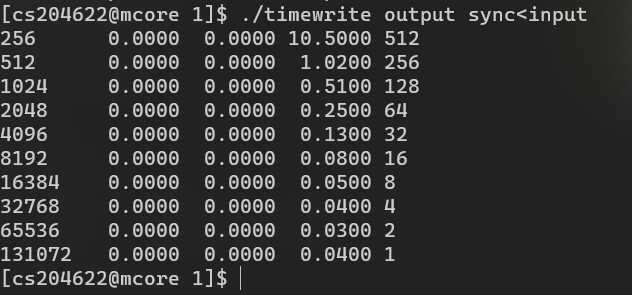
\includegraphics[width=0.4\textwidth]{output.png}
\end{figure}

不同平台的实验结果详细数据见\nameref{sec:appendix}

\section{实验结论}

\subsection{异步写在写入性能较差的介质和文件系统下有更强的加速效果}

WSL2中的Linux在写入Windows操作系统的分区时会出现较大的性能开销\cite{githubwsl2Filesystem}。
因此,借助WSL2中的Linux访问\textbf{WSL2映像中的文件}和访问\textbf{Windows操作系统分区中的文件}的对比,
可以反映出异步写入对效率的提升与存储介质和文件系统性能的关系。

为了直观地比较同步写入和异步写入的效率,在统计运行时间之外,还统计异步写入加速比率,计算方法如\eqref{eqn:acc}

\begin{equation}
	\label{eqn:acc}
	\mathop{\mathrm{acc}}=\frac{t_{sync}-t_{async}}{t_{sync}} \times 100\%
\end{equation}

结果如图~\ref{fig:acc}所示。

\begin{figure}[htbp]
	\centering
	\caption{异步写入加速比较}
	\label{fig:acc}
	\begin{subfigure}{0.4\textwidth}
		\centering
		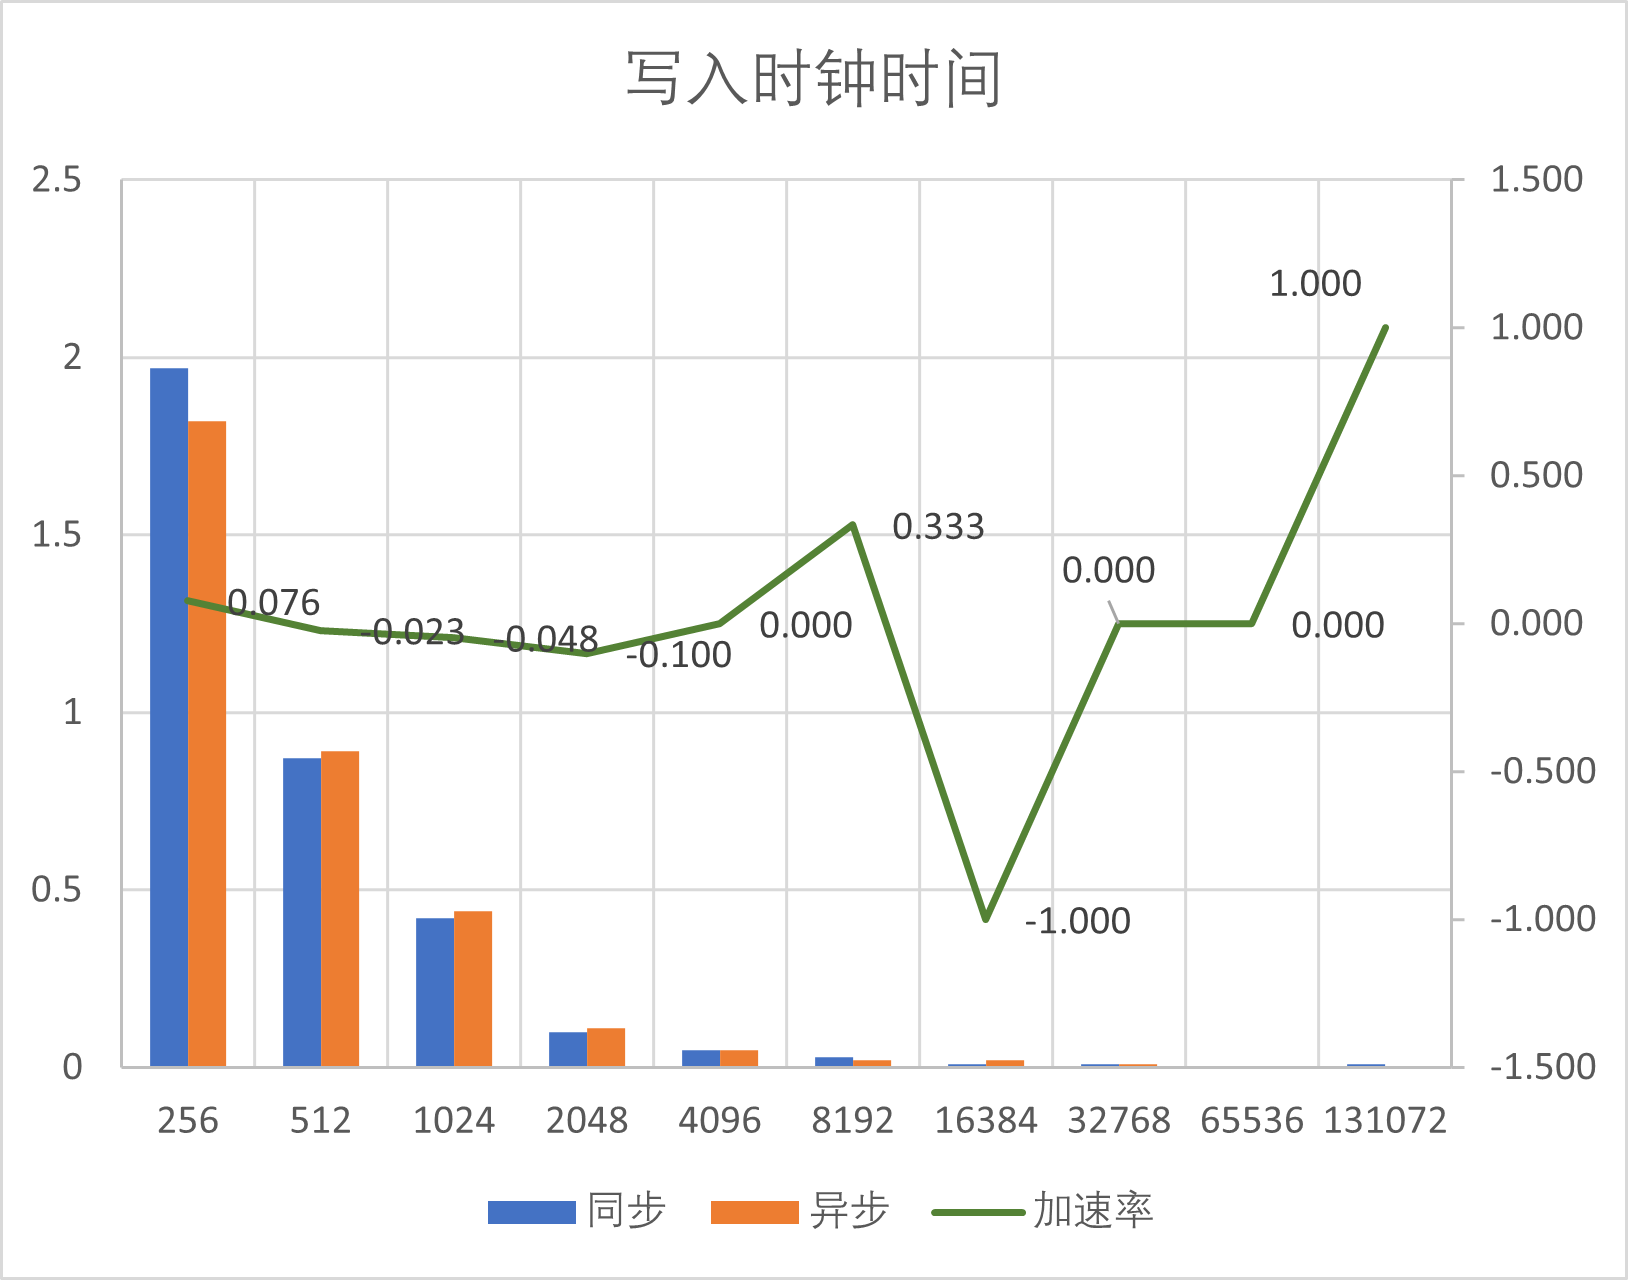
\includegraphics[width=\textwidth]{sync_async.png}
		\caption{WSL}
		\label{fig:wsl}
	\end{subfigure}
	\begin{subfigure}{0.4\textwidth}
		\centering
		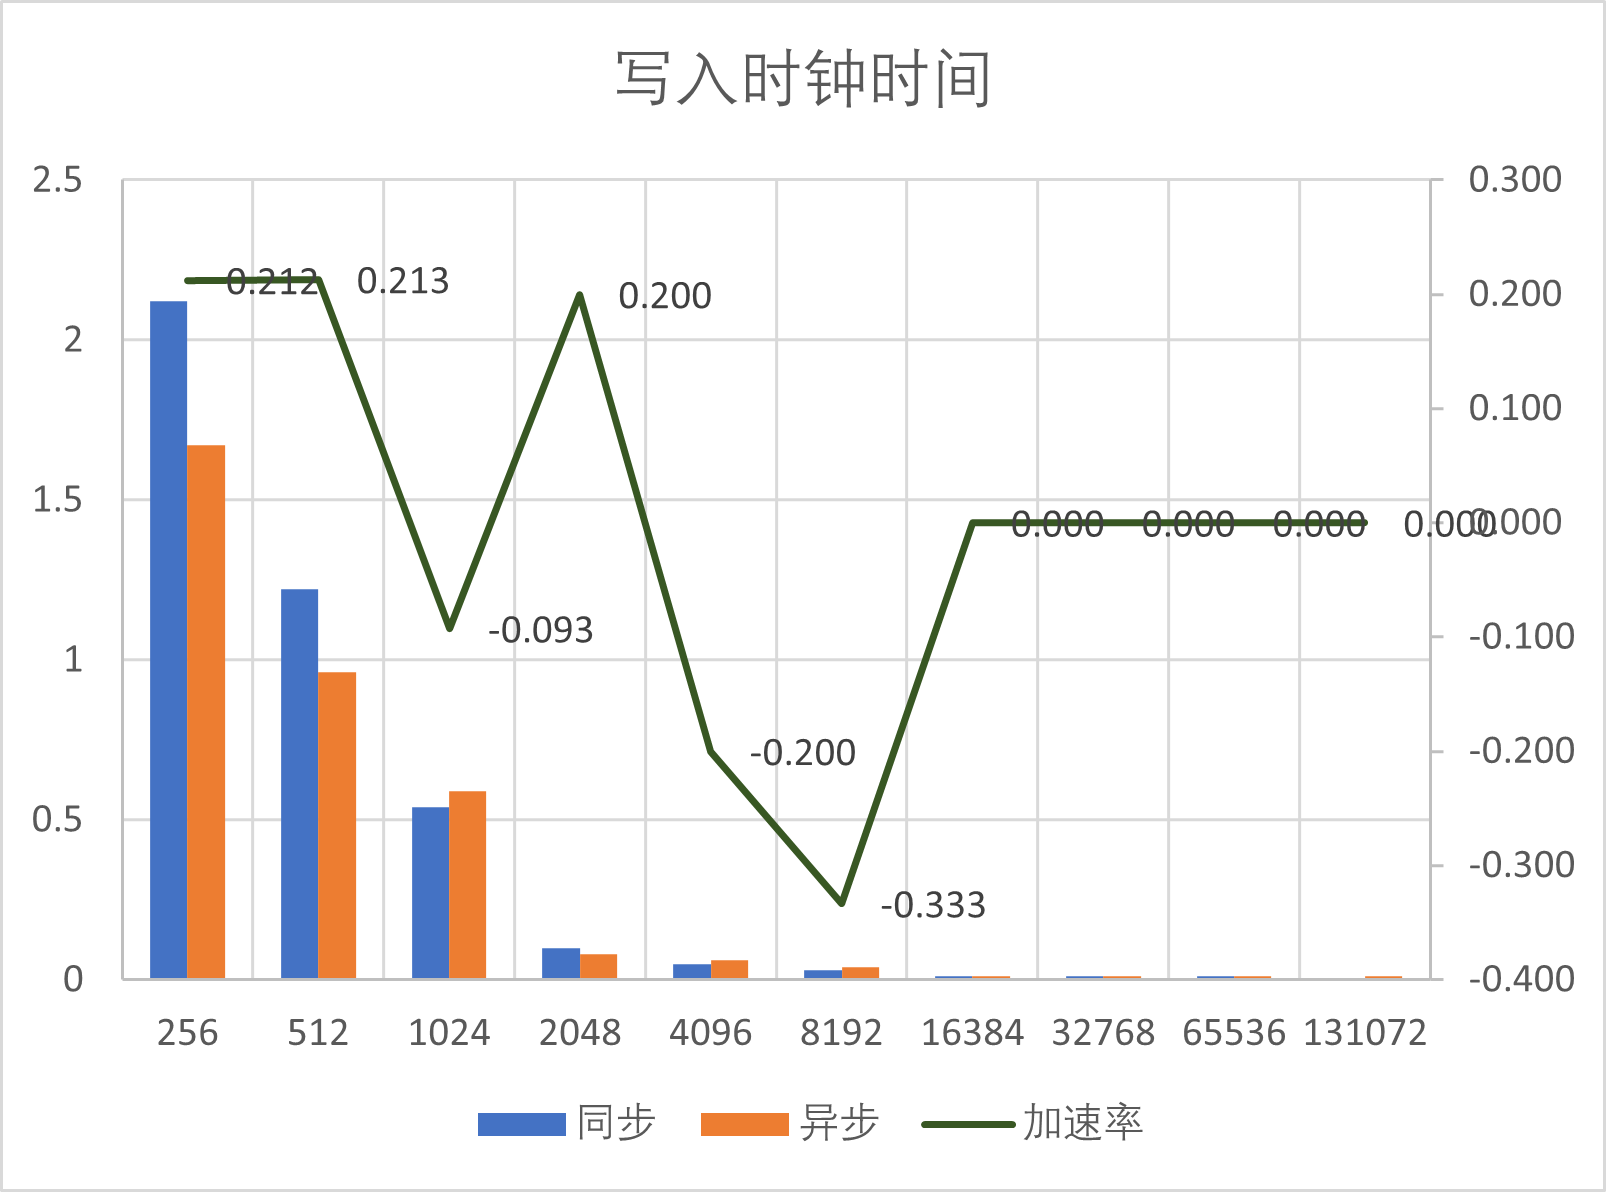
\includegraphics[width=\textwidth]{sync_async_slow.png}
		\caption{WSL(访问Windows文件系统)}
		\label{fig:wslwin}
	\end{subfigure}
\end{figure}

可以看出,在文件系统的读写效率较高、访问存储介质的性能能够充分发挥的情况下,异步写并不能带来
明显的性能提升,如图~\ref{fig:wsl}。然而当文件系统性能低下、访问存储介质的性能不佳时,异步写
能够对写入操作进行明显的加速。如图~\ref{fig:wslwin}。

随着每次写入数据量(BUFFSIZE)的增大,异步写入的加速能力下降,并在某一处值处开始转变为0贡献和负贡献。
这一阈值在文件系统的读写效率较高时来的更早(图~\ref{fig:wsl}),这侧面印证了异步写入对性能本身
较差的文件系统和存储介质的加速效果更好这一结论。

\subsection{FreeBSD上的ZFS文件系统确实有优秀的的性能表现}

BSD上的ZFS\cite{rodeh2003zfs}被证实具有良好的性能表现,不仅仅和ZFS on Linus相比,更能和EXT4等传统的
文件系统相比\cite{freebsdzfs}。本次实验也证明了一点。统计不同操作系统上同步写入的时钟时间,如图~\ref{fig:allsync}。

\begin{figure}[htb]
	\centering
	\caption{不同操作系统上同步写入的时钟时间}
	\label{fig:allsync}
	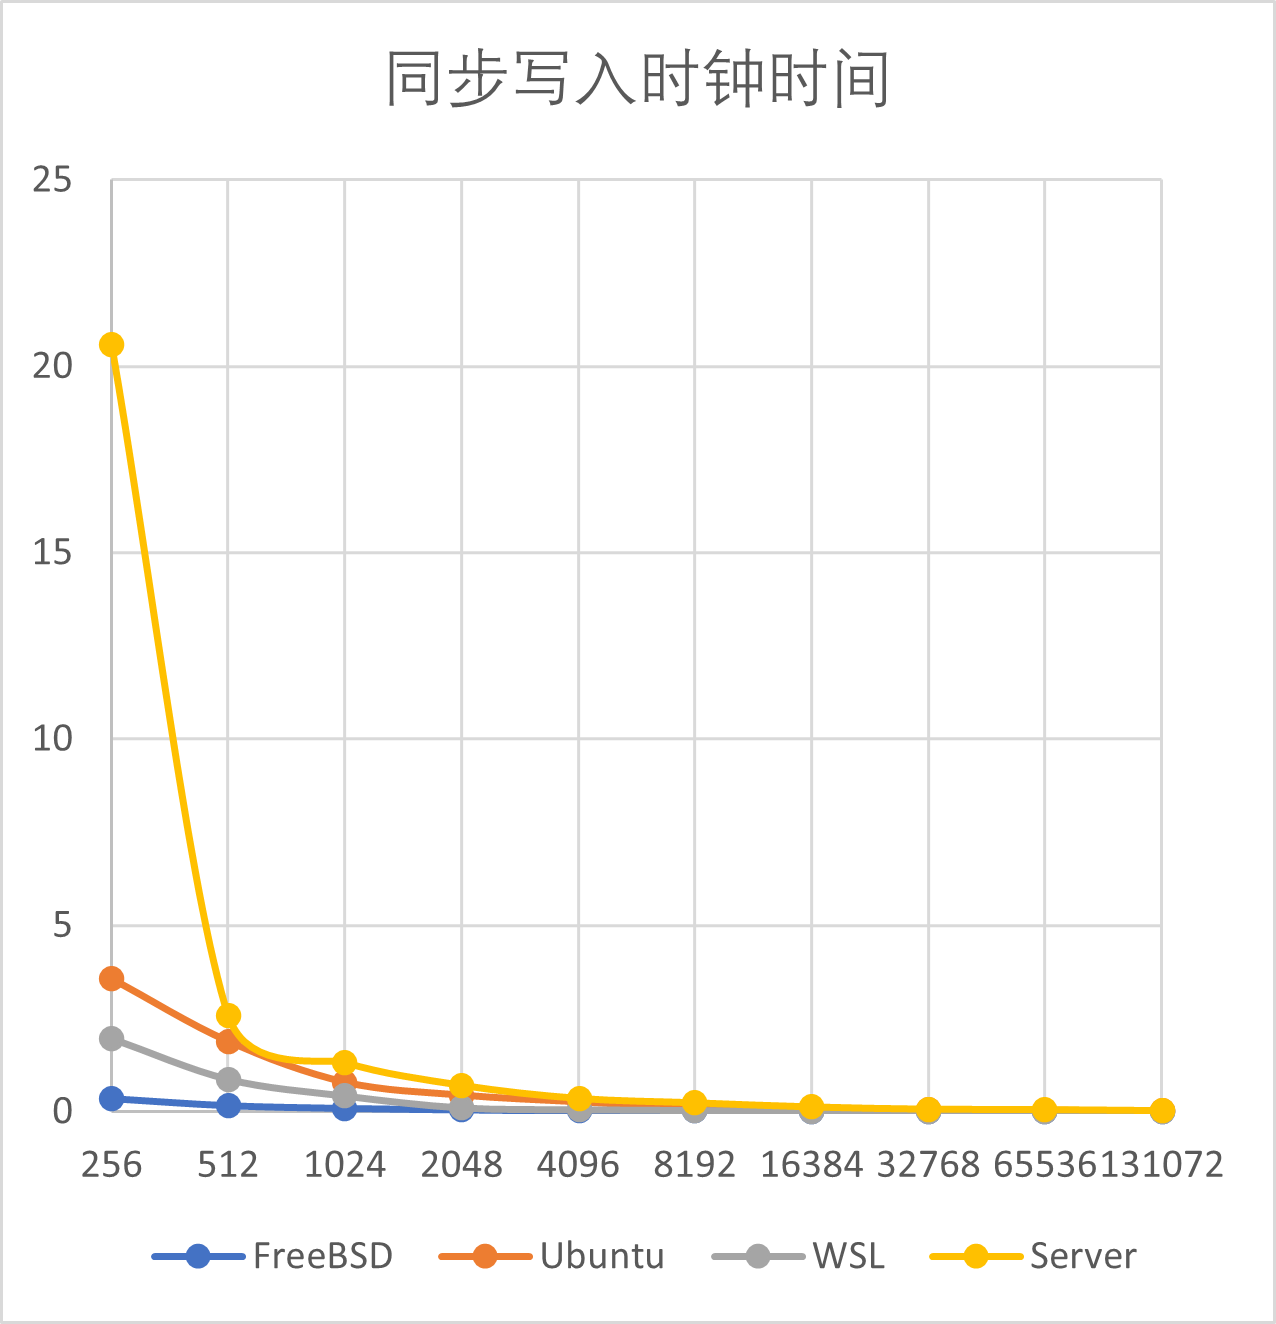
\includegraphics[width=0.4\textwidth]{clock.png}
\end{figure}

可见使用ZFS的FreeBSD有最好的性能表现,远好于其它对手。这一点也与\cite{freebsdzfs}的结论一致。因此,在维护和管理服务器时
我们应当采用先进技术,这样可以有效地提升性能。现如今IO瓶颈早已成为制约计算机性能的重要因素,因此采用性能良好的文件系统
意义重大。

\subsection{新的内核版本对减少系统调用开销有重大意义}

\begin{figure}[htb]
	\centering
	\caption{服务器上的Linux 2.6具有异常高的写入开销}
	\label{fig:highsync}
	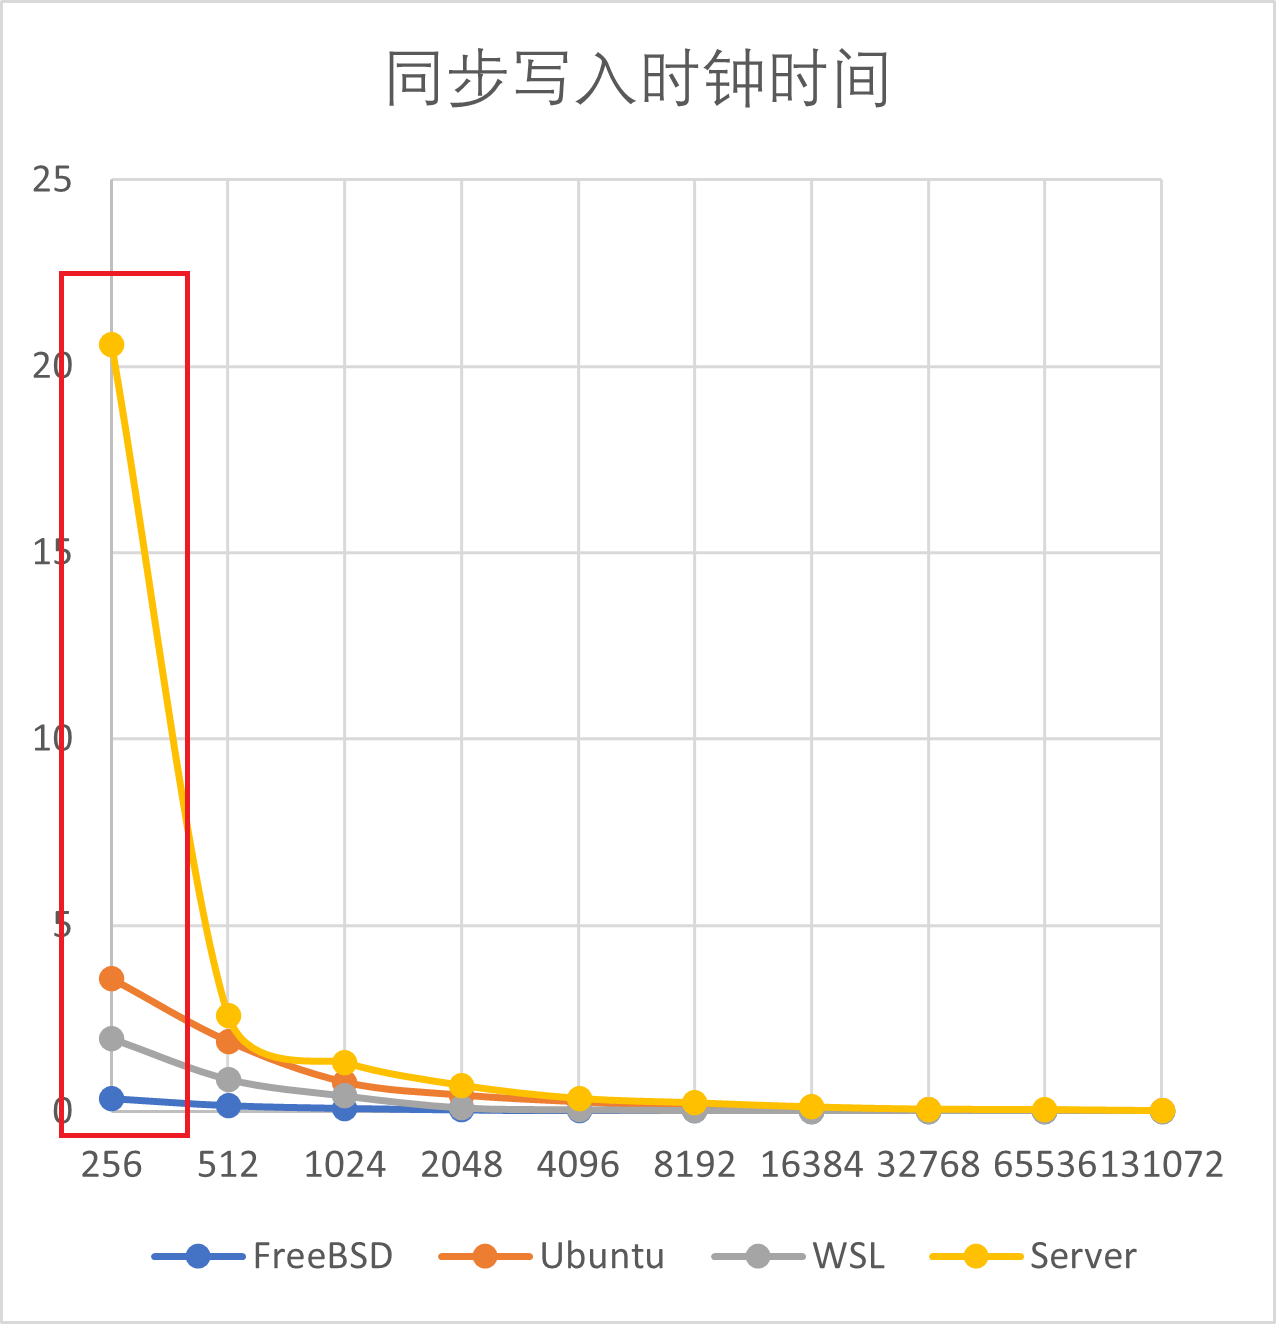
\includegraphics[width=0.4\textwidth]{clock_high.png}
\end{figure}

观察图~\ref{fig:highsync},可以发现在256的BUFFSIZE下,在学校服务器上运行该程序,写入时间相对而言特别长,而随着BUFFSIZE增加,
这种对比完全消失了。那么\textbf{这种异常的高开销的原因是什么呢?}

当BUFFSIZE为256时,需要调用512次\textbf{write()}才能写入全部数据,而每次调用\textbf{write()}都要进行系统调用。而从内核态切换到
用户态是有开销的。特别是当系统调用的实现方式比较传统时,该开销是相当可观的。

\subsubsection{Linux内核系统调用的实现}

自CPU引入保护模式以来,应用程序开始只能工作在具有诸多限制的用户态。为了允许应用程序实现那些需要更高特权级的指令具有的功能,需要一种
机制来允许应用程序进入内核态。这种机制在UNIX/类UNIX内核下就是系统调用。Linux内核的系统调用实现大致分为两个阶段。

\begin{itemize}
	\item \textbf{INT 80}  早期的Linux内核和当时绝大多数UNIX内核的系统调用都采用了软中断的形式。中断指令会自动将当前的状态保存在
	栈中,然后将控制权移交给运行在内核态的中断处理程序。在Linux内核中,使用的中断是\textbf{INT 0x80}。并且系统调用的调用者会把系统调用编号
	存储在EAX寄存器中。这样的机制的优点是系统调用的处理和中断的处理可以使用同一套机制,保存状态等过程实现简单。但是这种机制的缺点是并非所有的
	寄存器都需要保存,因此这个读写内存的过程大大降低了处理系统调用的效率。

	\item \textbf{sysenter/syexit和syscall/sysret}  sysenter/syexit和syscall/sysret分别由Intel\cite{guide2011intel}和AMD\cite{amd2018amd64}引入,
	用于快速地实现内核态和用户态的切换。它们没有寄存器状态入栈的内存操作,并且使用MSR寄存器来传递所需的信息。这样的机制有更高的性能。Linux内核在版本2.6中开始引入
	基于这些指令实现的系统调用机制。
\end{itemize}

在Linux内核上进行系统调用依赖GLibC库。考虑到Linux 2.6刚刚引入新的快速系统调用机制,我作出假设~\ref{ass:syscall}:

\begin{assumption}
	\label{ass:syscall}
	配套的GLibC库可能没有恰当地更新,以至于旧的系统调用机制仍然在使用,
	这意味着较高的开销,再加上BUFFSIZE为256时较多的调用次数,使得总体开销显得过高。
\end{assumption}

\subsubsection{实验验证}

为了验证这个猜想,我查阅了相应GLibC版本的源码。首先通过$ldd --version$命令获取了服务器上的GLibC版本是2.5。因此查找相应的分支的代码。
GLibC进行系统调用的源码位置位于\textbf{sysdeps/unix/sysv/linux/i386/sysdep.h}。该文件为i386架构的可执行文件提供系统调用的实现。
内容如图~\ref{fig:sysdepi386}。其中ENTER\_KERNEL的内容如图~\ref{fig:enterkernel}。

\begin{figure}[htbp]
	\centering
	\caption{GLibC的系统调用实现}
	\label{fig:acc}
	\begin{subfigure}{0.4\textwidth}
		\centering
		\caption{sysdep.h}
		\label{fig:sysdepi386}
		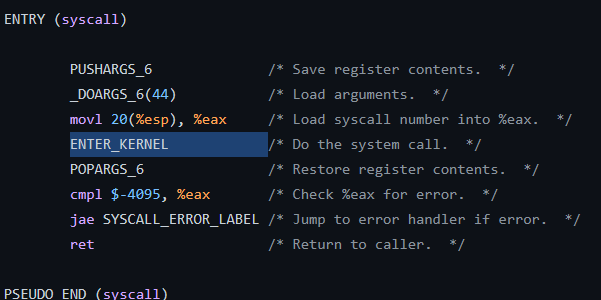
\includegraphics[width=\textwidth]{syscall_entry.png}
	\end{subfigure}
	\begin{subfigure}{0.4\textwidth}
		\centering
		\caption{ENTER\_KERNEL}
		\label{fig:enterkernel}
		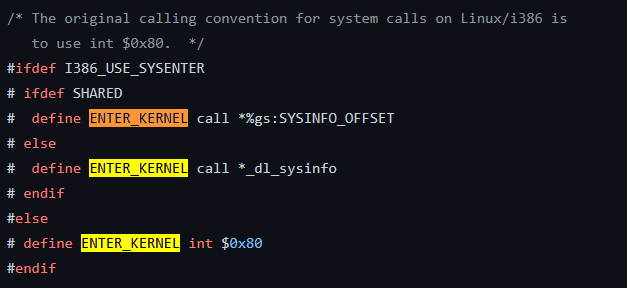
\includegraphics[width=\textwidth]{syscall.png}
	\end{subfigure}
\end{figure}

可见32位系统调用实现由编译参数定义的宏的不同,可能使用旧的INT80机制的,这可能带来
较大的开销。而对应的64位系统调用直接使用syscall/sysret指令组合,一定会
使用新的系统调用机制。

因此,为了验证猜想~\ref{ass:syscall},我重新编译了64位版本的timewrite,运行结果如图~\ref{fig:64bit}。
可以看出64位版本的timewrite的写入比32位版本快约50\%以上。从常识出发,这超出了字长的变化可能对性能带来的影响。
因此可以认为节省的时间是由于系统调用实现机制的不同而导致的效率区别,进而可以认为猜想~\ref{ass:syscall}是正确的。

\begin{figure}[htb]
	\centering
	\caption{64位版本与32位版本结果比较}
	\label{fig:64bit}
	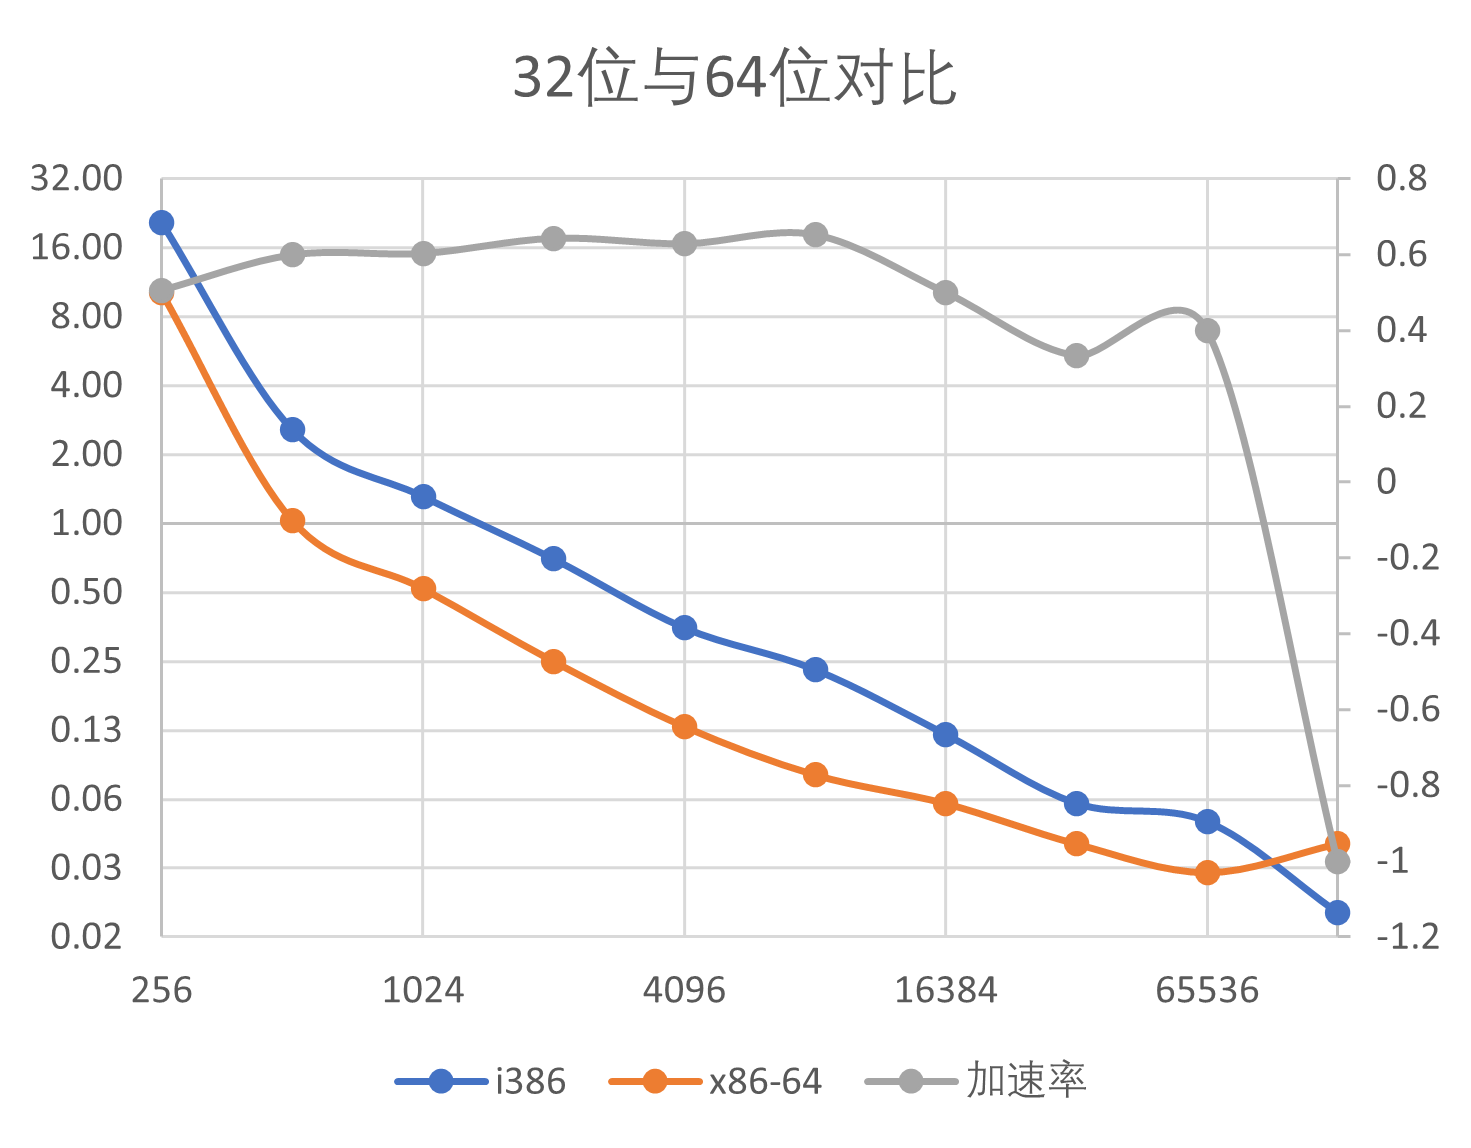
\includegraphics[width=0.4\textwidth]{64bit.png}
\end{figure}



\section{实验体会}

通过此次实验,我在5种不同平台、3种不同的操作系统下对同步写和异步写的效率进行了探究。

首先,我练习了UNIX下基础编程的技能。在日常的代码编写中,我通常使用CMake等高级的构建系统来完成
项目的组织和配置。通过这次实验,我又回顾了如何使用基础的Makefile组织项目文件、配置编译参数。并
实现了timewirte程序来测试同步写入和异步写入的性能。

其次,通过在不同的平台下运行该程序,我对同步写和异步写的效率差异和优劣有了感性的认识。在处理
实验数据的过程中,我练习了相应的图表绘制技巧和数据分析能力。

最后,为了验证对服务器上的Linux 2.6写入效率显著低下的原因的猜想,我查阅并分析了GLibC的开源代码
从开源代码中获得原因的提示,并进一步设计实验,通过不同架构链接的库具有差别的事实,验证了这个异常的
高开销可能是由于使用了具有较高开销的旧系统调用机制的原因。

\subsection{实验缺陷}

这次实验的过程也存在一定缺陷。例如课程服务器上的GCC 4.1版本过于老旧,因此无法与其他平台上的GCC 11
进行统一。由于GCC的开源许可证要求过于苛刻,FreeBSD上编译并安装GCC较为困难,因此使用的Clang编译器。
这对变量的控制产生的不利的影响。但是注意到该程序内容比较简单,同时没有启用较高的优化级别。因此这种
误差可以忽略不计。

\clearpage
\section*{参考文献}
\addcontentsline{toc}{part}{参考文献}

\bibliographystyle{unsrt}
\bibliography{reference}

\clearpage
\section*{附录:代码清单}
\addcontentsline{toc}{part}{附录:代码清单}
\label{sec:code}

\subsection{Makefile}


\begin{lstlisting}[numbers=left,style=MakefileStyle,caption=Makefile,label={code:makefile}]
OUT = build
SRC = .
CC = gcc
LD = ld

all: timewrite

${OUT}: 
	mkdir -p $(OUT)

${OUT}/timewrite.o: ${OUT} $(SRC)/timewrite.c
	$(CC) -std=c99 -c $(SRC)/timewrite.c -o $(OUT)/timewrite.o

timewrite: $(OUT)/timewrite.o
	$(CC) $(OUT)/timewrite.o -o timewrite

clean: 
	rm -rf $(OUT) timewrite

.PHONY: all clean	
\end{lstlisting}


\subsection{程序实现}

\begin{lstlisting}[numbers=left,style=CppStyle,caption=程序实现,label={code:impl}]
#include <sys/times.h>
#include <unistd.h>
#include <fcntl.h>

#include <stdio.h>
#include <assert.h>
#include <string.h>
#include <stdlib.h>

#define FILE_MODE (S_IRUSR | S_IWUSR | S_IRGRP | S_IROTH)


int main(int argc, char** argv)
{
    assert(argc == 2 || argc == 3);

    if (argc == 3 && strcmp(argv[2], "sync") != 0)
    {
        printf("usage: %s <pathname> [sync]", argv[0]);
        return 1;
    }

    const int mode = (argc == 3) ? O_RDWR | O_CREAT | O_TRUNC | O_SYNC : O_RDWR | O_CREAT | O_TRUNC;

    int out_file = open(argv[1], mode, FILE_MODE);
    if (out_file < 0)
    {
        printf("open error");
        return 1;
    }

    int length = lseek(STDIN_FILENO, 0, SEEK_END);
    if (length < 0)
    {
        printf("lseek error");
        return 1;
    }

    if (lseek(STDIN_FILENO, 0, SEEK_SET) < 0)
    {
        printf("lseek error");
        return 1;
    }

    char* buff = malloc(length);
    if (buff == NULL)
    {
        printf("malloc error");
        return 1;
    }

    if (read(STDIN_FILENO, buff, length) != length)
    {
        printf("read error");
        return 1;
    }

    const int lock_per_second = sysconf(_SC_CLK_TCK);

    for (int bufsize = 256;bufsize <= 131072;bufsize <<= 1)
    {
        lseek(out_file, 0, SEEK_SET);

        int g = length / bufsize, res = length % bufsize;
        struct tms start, end;
        clock_t start_clock, end_clock;
        start_clock = times(&start);
        
        for (int i = 0;i < g;i++)
        {
            if (write(out_file, buff + i * bufsize, bufsize) != bufsize)
            {
                printf("write error");
                return 1;
            }
        }

        if (res != 0 && write(out_file, buff + g * bufsize, res) != res)
        {
            printf("write error");
            return 1;
        }
        end_clock = times(&end);

        const int loop = g + (res != 0);
        const double real_time = (double)(end_clock - start_clock) / lock_per_second;
        const double user_time = (double)(end.tms_utime - start.tms_utime) / lock_per_second;
        const double sys_time = (double)(end.tms_stime - start.tms_stime) / lock_per_second;

        printf("%d\t%7.4lf\t%7.4lf\t%7.4lf\t%d\n", bufsize, user_time, sys_time,real_time, loop);

    }

    return 0;
}
\end{lstlisting}

\clearpage
\section*{附录:实验详细数据}
\addcontentsline{toc}{part}{附录:实验详细数据}
\label{sec:appendix}

\subsection{WSL上的Ubuntu}

\begin{table}[H]
\centering
\caption{同步写入}
\begin{tabular}{c|c|c|c|c}
	\toprule
	\hline
	BUFFSIZE & 用户时间 & 系统时间 & 时钟时间 & 循环次数 \\
	\hline
	256      &0.0000&  0.1900&  1.9700& 5120
	\\512      &0.0000&  0.0900&  0.8700& 2560
	\\1024     &0.0000&  0.0500&  0.4200& 1280
	\\2048     &0.0000&  0.0000&  0.1000& 640
	\\4096     &0.0000&  0.0100&  0.0500& 320
	\\8192     &0.0000&  0.0000&  0.0300& 160
	\\16384    &0.0000&  0.0000&  0.0100& 80
	\\32768    &0.0000&  0.0000&  0.0100& 40
	\\65536    &0.0000&  0.0000&  0.0000& 20
	\\131072   &0.0000&  0.0000&  0.0100& 10\\
	\hline
	\bottomrule
\end{tabular}	
\end{table}

\begin{table}[H]
\centering
\caption{异步写入}
\begin{tabular}{c|c|c|c|c}
	\toprule
	\hline
	BUFFSIZE & 用户时间 & 系统时间 & 时钟时间 & 循环次数 \\
	\hline
	\\256    &  0.0000 & 0.1700 & 1.8200 & 5120
	\\512    &  0.0000 & 0.0800 & 0.8900 & 2560
	\\1024   &  0.0000 & 0.0400 & 0.4400 & 1280
	\\2048   &  0.0000 & 0.0100 & 0.1100 & 640
	\\4096   &  0.0000 & 0.0000 & 0.0500 & 320
	\\8192   &  0.0000 & 0.0000 & 0.0200 & 160
	\\16384  &  0.0000 & 0.0000 & 0.0200 & 80
	\\32768  &  0.0000 & 0.0000 & 0.0100 & 40
	\\65536  &  0.0000 & 0.0000 & 0.0000 & 20
	\\131072 &  0.0100 & 0.0000 & 0.0000 & 10\\
	\hline
	\bottomrule
\end{tabular}	
\end{table}

\subsection{WSL上的Ubuntu(访问Windows文件系统)}

\begin{table}[H]
\centering
\caption{同步写入}
\begin{tabular}{c|c|c|c|c}
	\toprule
	\hline
	BUFFSIZE & 用户时间 & 系统时间 & 时钟时间 & 循环次数 \\
	\hline
	256     & 0.0000 & 0.1600 & 1.6700& 5120
	\\512     & 0.0000 & 0.1200 & 0.9600& 2560
	\\1024    & 0.0000 & 0.1000 & 0.5900& 1280
	\\2048    & 0.0000 & 0.0100 & 0.0800& 640
	\\4096    & 0.0000 & 0.0100 & 0.0600& 320
	\\8192    & 0.0000 & 0.0000 & 0.0400& 160
	\\16384   & 0.0000 & 0.0000 & 0.0100& 80
	\\32768   & 0.0000 & 0.0000 & 0.0100& 40
	\\65536   & 0.0000 & 0.0000 & 0.0100& 20
	\\131072  & 0.0000 & 0.0000 & 0.0100& 10
	\\\hline
	\bottomrule
\end{tabular}	
\end{table}

\begin{table}[H]
\centering
\caption{异步写入}
\begin{tabular}{c|c|c|c|c}
	\toprule
	\hline
	BUFFSIZE & 用户时间 & 系统时间 & 时钟时间 & 循环次数 \\
	\hline
	256    &  0.0000 & 0.2900 & 2.1200 & 5120
	\\512    &  0.0100 & 0.1800 & 1.2200 & 2560
	\\1024   &  0.0000 & 0.0700 & 0.5400 & 1280
	\\2048   &  0.0000 & 0.0100 & 0.1000 & 640
	\\4096   &  0.0000 & 0.0000 & 0.0500 & 320
	\\8192   &  0.0000 & 0.0000 & 0.0300 & 160
	\\16384  &  0.0000 & 0.0000 & 0.0100 & 80
	\\32768  &  0.0000 & 0.0000 & 0.0100 & 40
	\\65536  &  0.0000 & 0.0000 & 0.0100 & 20
	\\131072 &  0.0000 & 0.0000 & 0.0000 & 10
	\\\hline
	\bottomrule
\end{tabular}	
\end{table}

\subsection{VMWare上的Ubuntu}


\begin{table}[H]
\centering
\caption{同步写入}
\begin{tabular}{c|c|c|c|c}
	\toprule
	\hline
	BUFFSIZE & 用户时间 & 系统时间 & 时钟时间 & 循环次数 \\
	\hline
	256   &   0.0100 & 0.7700 & 3.5800 & 5120
	\\512   &   0.0100 & 0.4000 & 1.8900 & 2560
	\\1024  &   0.0000 & 0.1600 & 0.7900 & 1280
	\\2048  &   0.0000 & 0.1000 & 0.4400 & 640
	\\4096  &   0.0000 & 0.0600 & 0.2600 & 320
	\\8192  &   0.0000 & 0.0200 & 0.1000 & 160
	\\16384 &   0.0000 & 0.0200 & 0.0700 & 80
	\\32768 &   0.0000 & 0.0000 & 0.0400 & 40
	\\65536 &   0.0000 & 0.0100 & 0.0300 & 20
	\\131072&   0.0000 & 0.0000 & 0.0200 & 10
	\\\hline
	\bottomrule
\end{tabular}	
\end{table}

\begin{table}[H]
\centering
\caption{异步写入}
\begin{tabular}{c|c|c|c|c}
	\toprule
	\hline
	BUFFSIZE & 用户时间 & 系统时间 & 时钟时间 & 循环次数 \\
	\hline
	256    &  0.0000 & 0.0400 & 0.0500 & 5120
	\\512    &  0.0000 & 0.0300 & 0.0300 & 2560
	\\1024   &  0.0000 & 0.0100 & 0.0000 & 1280
	\\2048   &  0.0000 & 0.0000 & 0.0100 & 640
	\\4096   &  0.0100 & 0.0000 & 0.0100 & 320
	\\8192   &  0.0000 & 0.0100 & 0.0000 & 160
	\\16384  &  0.0000 & 0.0000 & 0.0000 & 80
	\\32768  &  0.0000 & 0.0000 & 0.0000 & 40
	\\65536  &  0.0000 & 0.0000 & 0.0000 & 20
	\\131072 &  0.0000 & 0.0000 & 0.0000 & 10
	\\\hline
	\bottomrule
\end{tabular}	
\end{table}


\subsection{VMWare上的FreeBSD}


\begin{table}[H]
\centering
\caption{同步写入}
\begin{tabular}{c|c|c|c|c}
	\toprule
	\hline
	BUFFSIZE & 用户时间 & 系统时间 & 时钟时间 & 循环次数 \\
	\hline
	256	     &0.0000	 &0.0625	 &0.3594	&512
	\\512	     &0.0000	 &0.0234	 &0.1641	&256
	\\1024	 &0.0000	 &0.0156	 &0.0859	&128
	\\2048	 &0.0000	 &0.0078	 &0.0469	&64
	\\4096	 &0.0000	 &0.0078	 &0.0156	&32
	\\8192	 &0.0000	 &0.0000	 &0.0156	&16
	\\16384	 &0.0000	 &0.0000	 &0.0078	&8
	\\32768	 &0.0000	 &0.0000	 &0.0000	&4
	\\65536	 &0.0000	 &0.0000	 &0.0000	&2
	\\131072	 &0.0000	 &0.0000	 &0.0000	&1
	\\\hline
	\bottomrule
\end{tabular}	
\end{table}

\begin{table}[H]
\centering
\caption{异步写入}
\begin{tabular}{c|c|c|c|c}
	\toprule
	\hline
	BUFFSIZE & 用户时间 & 系统时间 & 时钟时间 & 循环次数 \\
	\hline
	256	 	 &0.0000	 &0.0000	 &0.0000	&512
	\\512	 	 &0.0000	 &0.0000	 &0.0000	&256
	\\1024	 &0.0000	 &0.0000	 &0.0000	&128
	\\2048	 &0.0000	 &0.0000	 &0.0000	&64
	\\4096	 &0.0000	 &0.0000	 &0.0000	&32
	\\8192	 &0.0000	 &0.0000	 &0.0000	&16
	\\16384	 &0.0000	 &0.0000	 &0.0000	&8
	\\32768	 &0.0000	 &0.0000	 &0.0000	&4
	\\65536	 &0.0000	 &0.0000	 &0.0000	&2
	\\131072	 &0.0000	 &0.0000	 &0.0000	&1
	\\\hline
	\bottomrule
\end{tabular}	
\end{table}

\subsection{服务器上的Linux 2.6}



\begin{table}[H]
\centering
\caption{同步写入}
\begin{tabular}{c|c|c|c|c}
	\toprule
	\hline
	BUFFSIZE & 用户时间 & 系统时间 & 时钟时间 & 循环次数 \\
	\hline
	256    &  0.0000 & 0.0200 &20.5800 &512
	\\512    &  0.0000 & 0.0100 & 2.5700 &256
	\\1024   &  0.0000 & 0.0000 & 1.3100 &128
	\\2048   &  0.0000 & 0.0000 & 0.7000 &64
	\\4096   &  0.0000 & 0.0000 & 0.3500 &32
	\\8192   &  0.0000 & 0.0000 & 0.2300 &16
	\\16384  &  0.0000 & 0.0000 & 0.1200 &8
	\\32768  &  0.0000 & 0.0000 & 0.0600 &4
	\\65536  &  0.0000 & 0.0000 & 0.0500 &2
	\\131072 &  0.0000 & 0.0000 & 0.0200 &1
	\\\hline
	\bottomrule
\end{tabular}	
\end{table}

\begin{table}[H]
\centering
\caption{异步写入}
\begin{tabular}{c|c|c|c|c}
	\toprule
	\hline
	BUFFSIZE & 用户时间 & 系统时间 & 时钟时间 & 循环次数 \\
	\hline
	256     & 0.0000 & 0.0000 & 0.0000 & 512
	\\512     & 0.0000 & 0.0000 & 0.0000 & 256
	\\1024    & 0.0000 & 0.0000 & 0.0000 & 128
	\\2048    & 0.0000 & 0.0000 & 0.0000 & 64
	\\4096    & 0.0000 & 0.0000 & 0.0000 & 32
	\\8192    & 0.0000 & 0.0000 & 0.0000 & 16
	\\16384   & 0.0000 & 0.0000 & 0.0000 & 8
	\\32768   & 0.0000 & 0.0000 & 0.0000 & 4
	\\65536   & 0.0000 & 0.0000 & 0.0000 & 2
	\\131072  & 0.0000 & 0.0000 & 0.0000 & 1
	\\\hline
	\bottomrule
\end{tabular}	
\end{table}

\end{spacing}

\end{document}